\section{\ttt{2D} Classification}
 \begin{figure}[H]
  \centering
  \captionsetup{width=.8\linewidth} 
  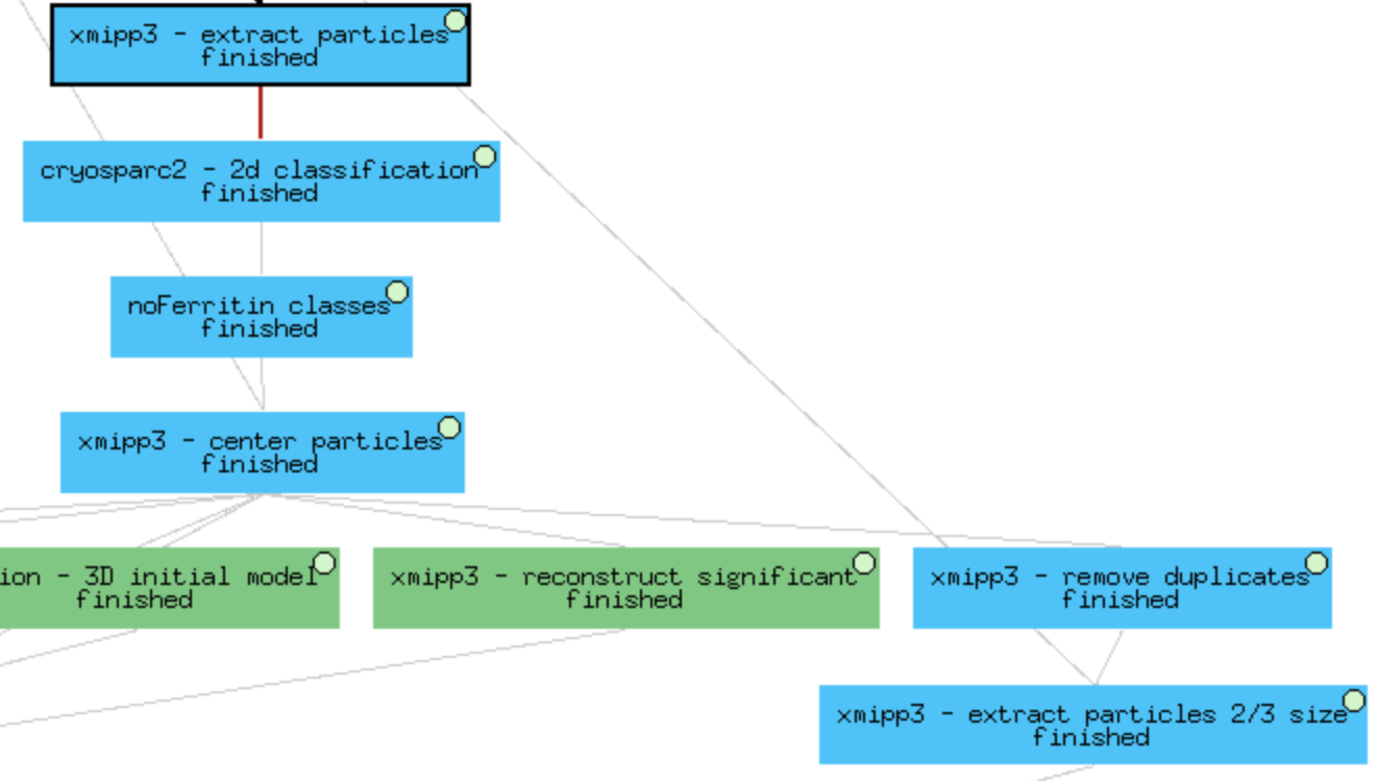
\includegraphics[width=0.95\textwidth]
  {{images/7_workflow5_2DClassification.pdf}}
  \caption{\ttt{2D} classification workflow (Blue color).}
  \label{fig:workflow_5}
  \end{figure}
  
The next step in image processing involves the \ttt{2D} classification of particle images to group similar ones. This process can serve as an exploratory tool of your data and might also be used to throw away bad particles. In addition, by overlapping similar images we can obtain the average images or \ttt{2D} classes. Since these classes are the projections of the 3D object that we try to reconstruct, they can also be used in the reconstruction of the 3D object.\\

Although there exist several \ttt{2D} classification algorithms, in this tutorial the \ttt{2D} classes will be created with the $cryoSPARC$ \citep{punjani2017cryosparc} \ttt{2D} classification method \citep{punjani2016building}, integrated in the protocol \scommand{cryosparc2-2D classification}. We used as input the subset of particles previously selected. The \ttt{2D} classification parameters can be observed in the central tap of the protocol form in the \ffigure{fig:cryosparc2_second_tap}. Remark that we choose in advance the number of classes, 50 in this case.

\begin{figure}[H]
  \centering
  \captionsetup{width=.8\linewidth} 
  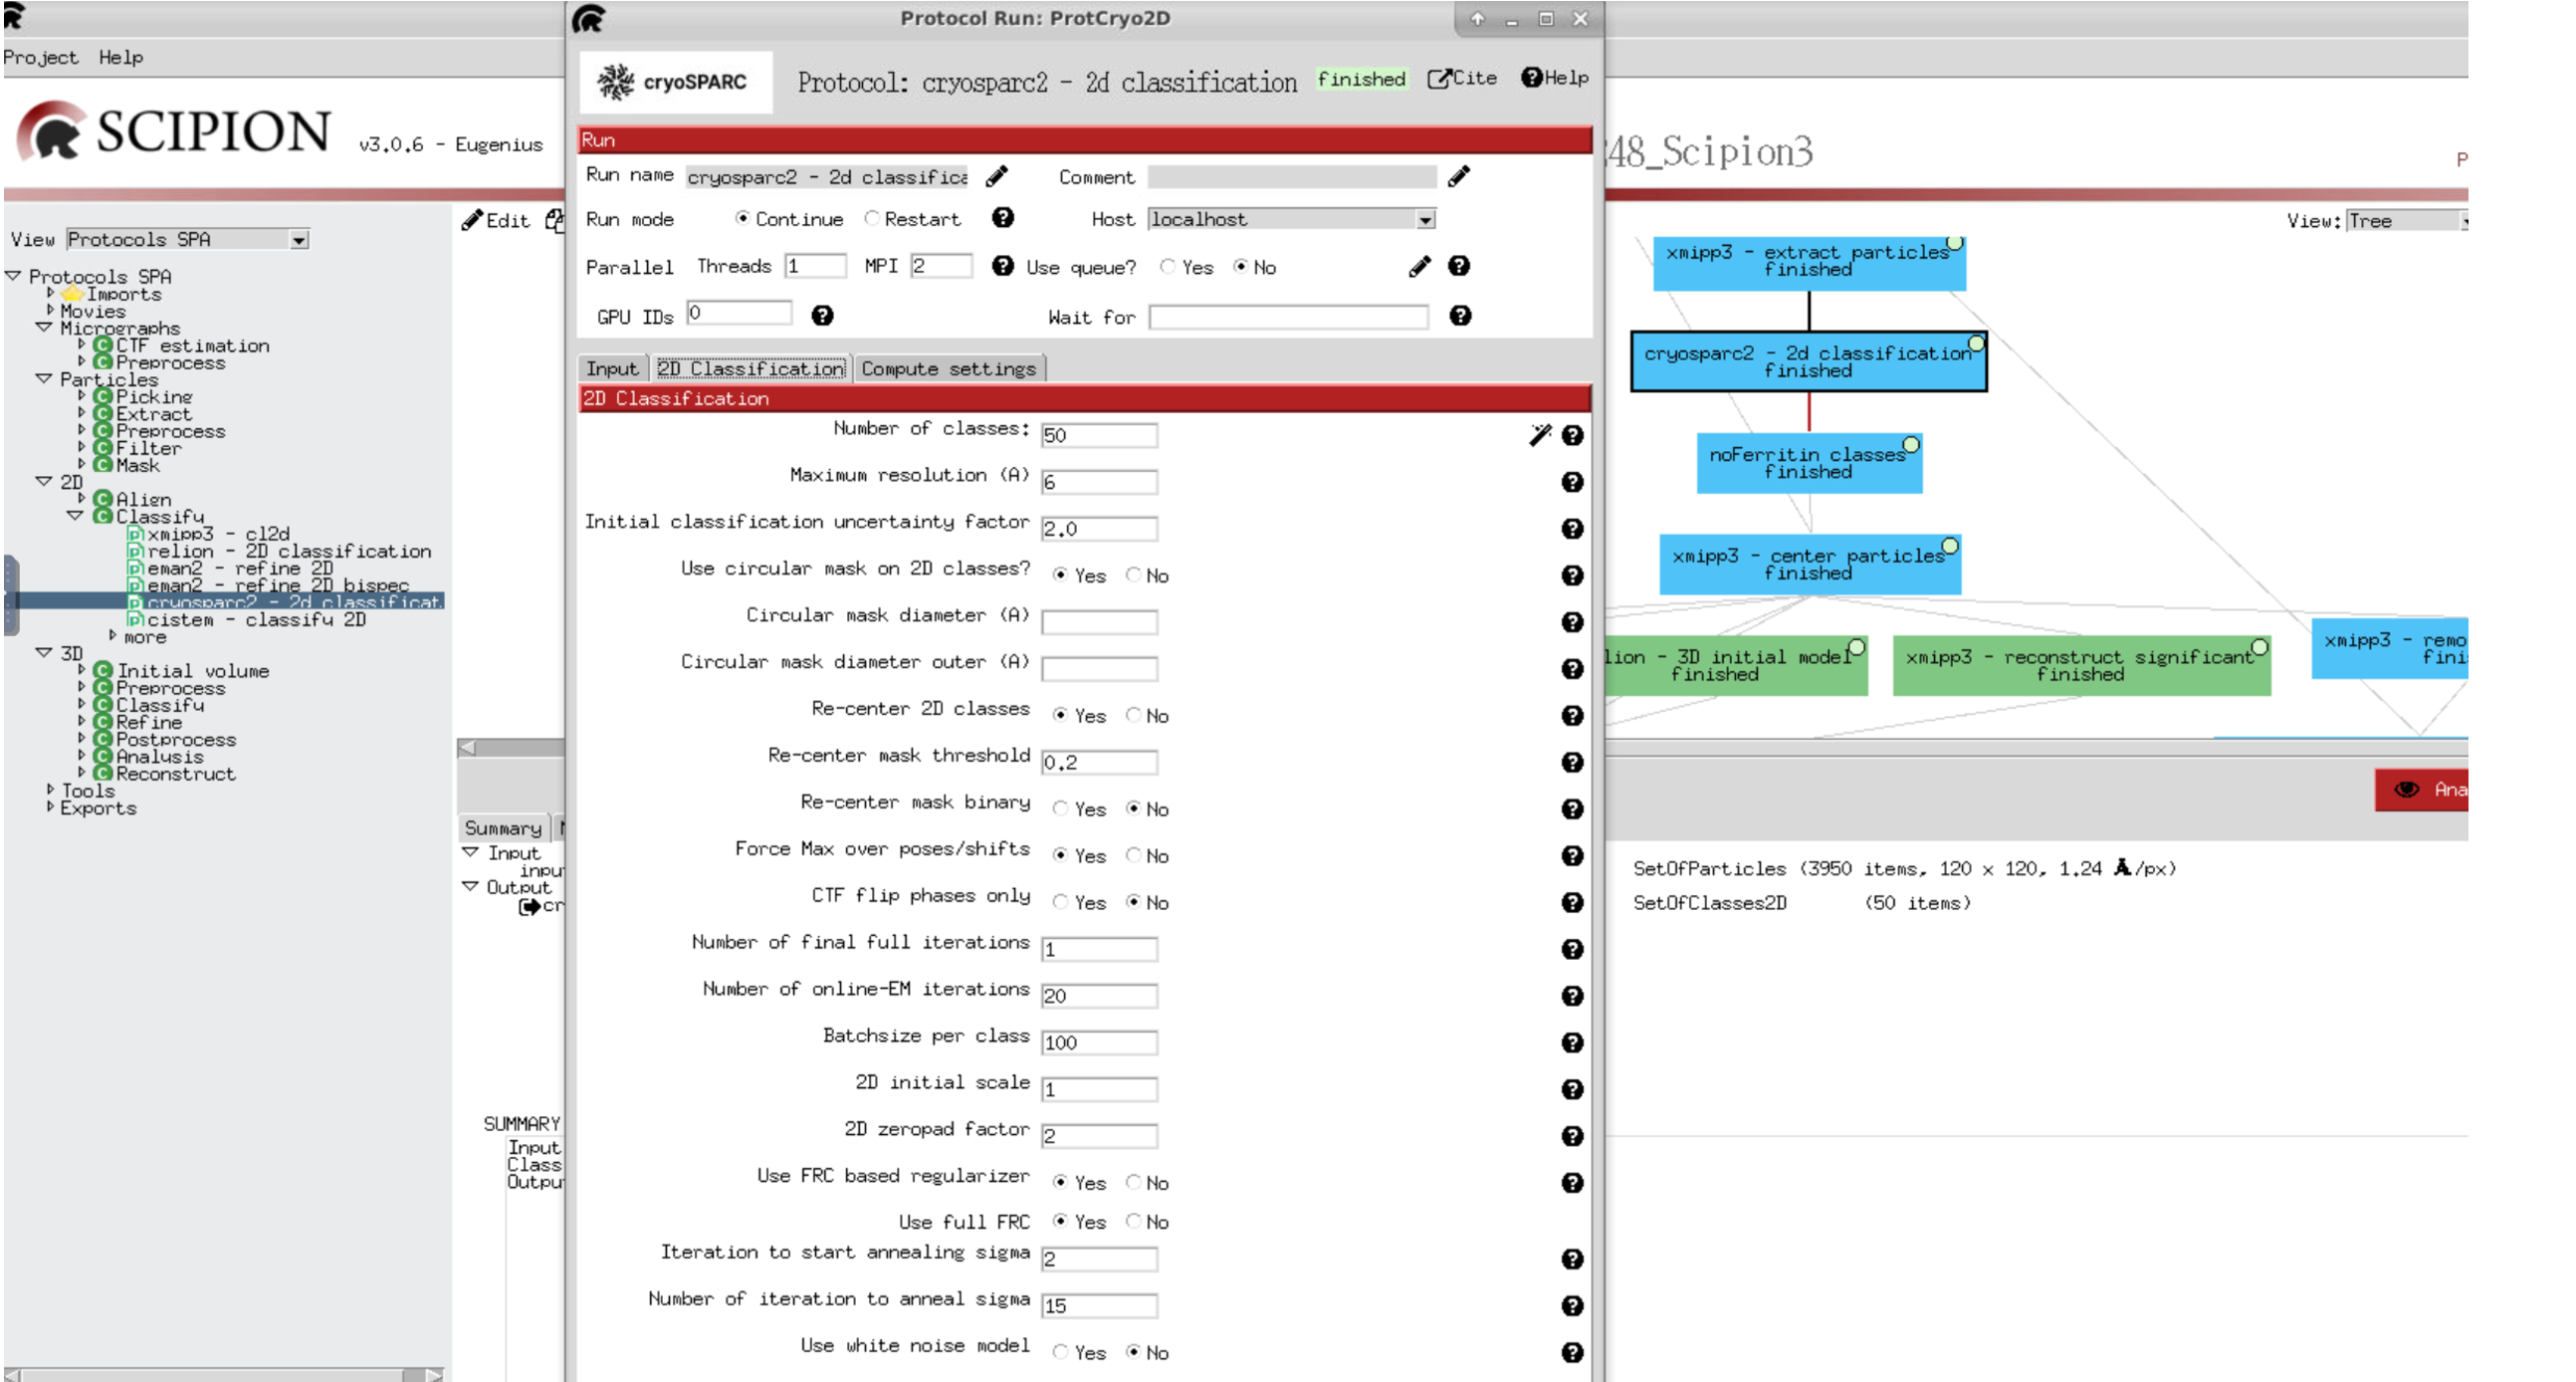
\includegraphics[width=0.95\textwidth]
  {images/7a_cryosparc2_2DClass.pdf}
  \caption{Filling in the second tap of the protocol \scommand{cryosparc2-2D classification}.}
  \label{fig:cryosparc2_second_tap}
  \end{figure}
  
After running the protocol, particle classes can be visualized selecting any of the two options of the menu opened with \scommand{Analyze Results}, the common \scipion viewer or the $cryoSPARC$ GUI. By double-clicking or right-clicking the classes we can see the particles behind those classes. The final number of classes also appears in the Summary output, which in this case is 50 classes. \\

Once inspected the different classes, in \scipion we can discard manually the ones that still have the iron attached (Ferritin molecules), which will appear as a white dot in the core of the particle. In our case we found that 378 particles had the iron attached. Then by selecting the classes that we are interested in (38 from 50) and pressing \scommand{Classes}, a new set of 38 Classes, which contained both the average (class representative particles) and the particles behind them (3,491), will be created included in the box \ttt{noFerritin classes}.\\  

The next protocol \scommand{xmipp3-center particles} will recenter the particles. For centering the particles, we needed as input both the classes and the set of micrographs, as we can see in the protocol form \ffigure{fig:xmipp3_centParticles}.  

\begin{figure}[H]
  \centering
  \captionsetup{width=.8\linewidth} 
  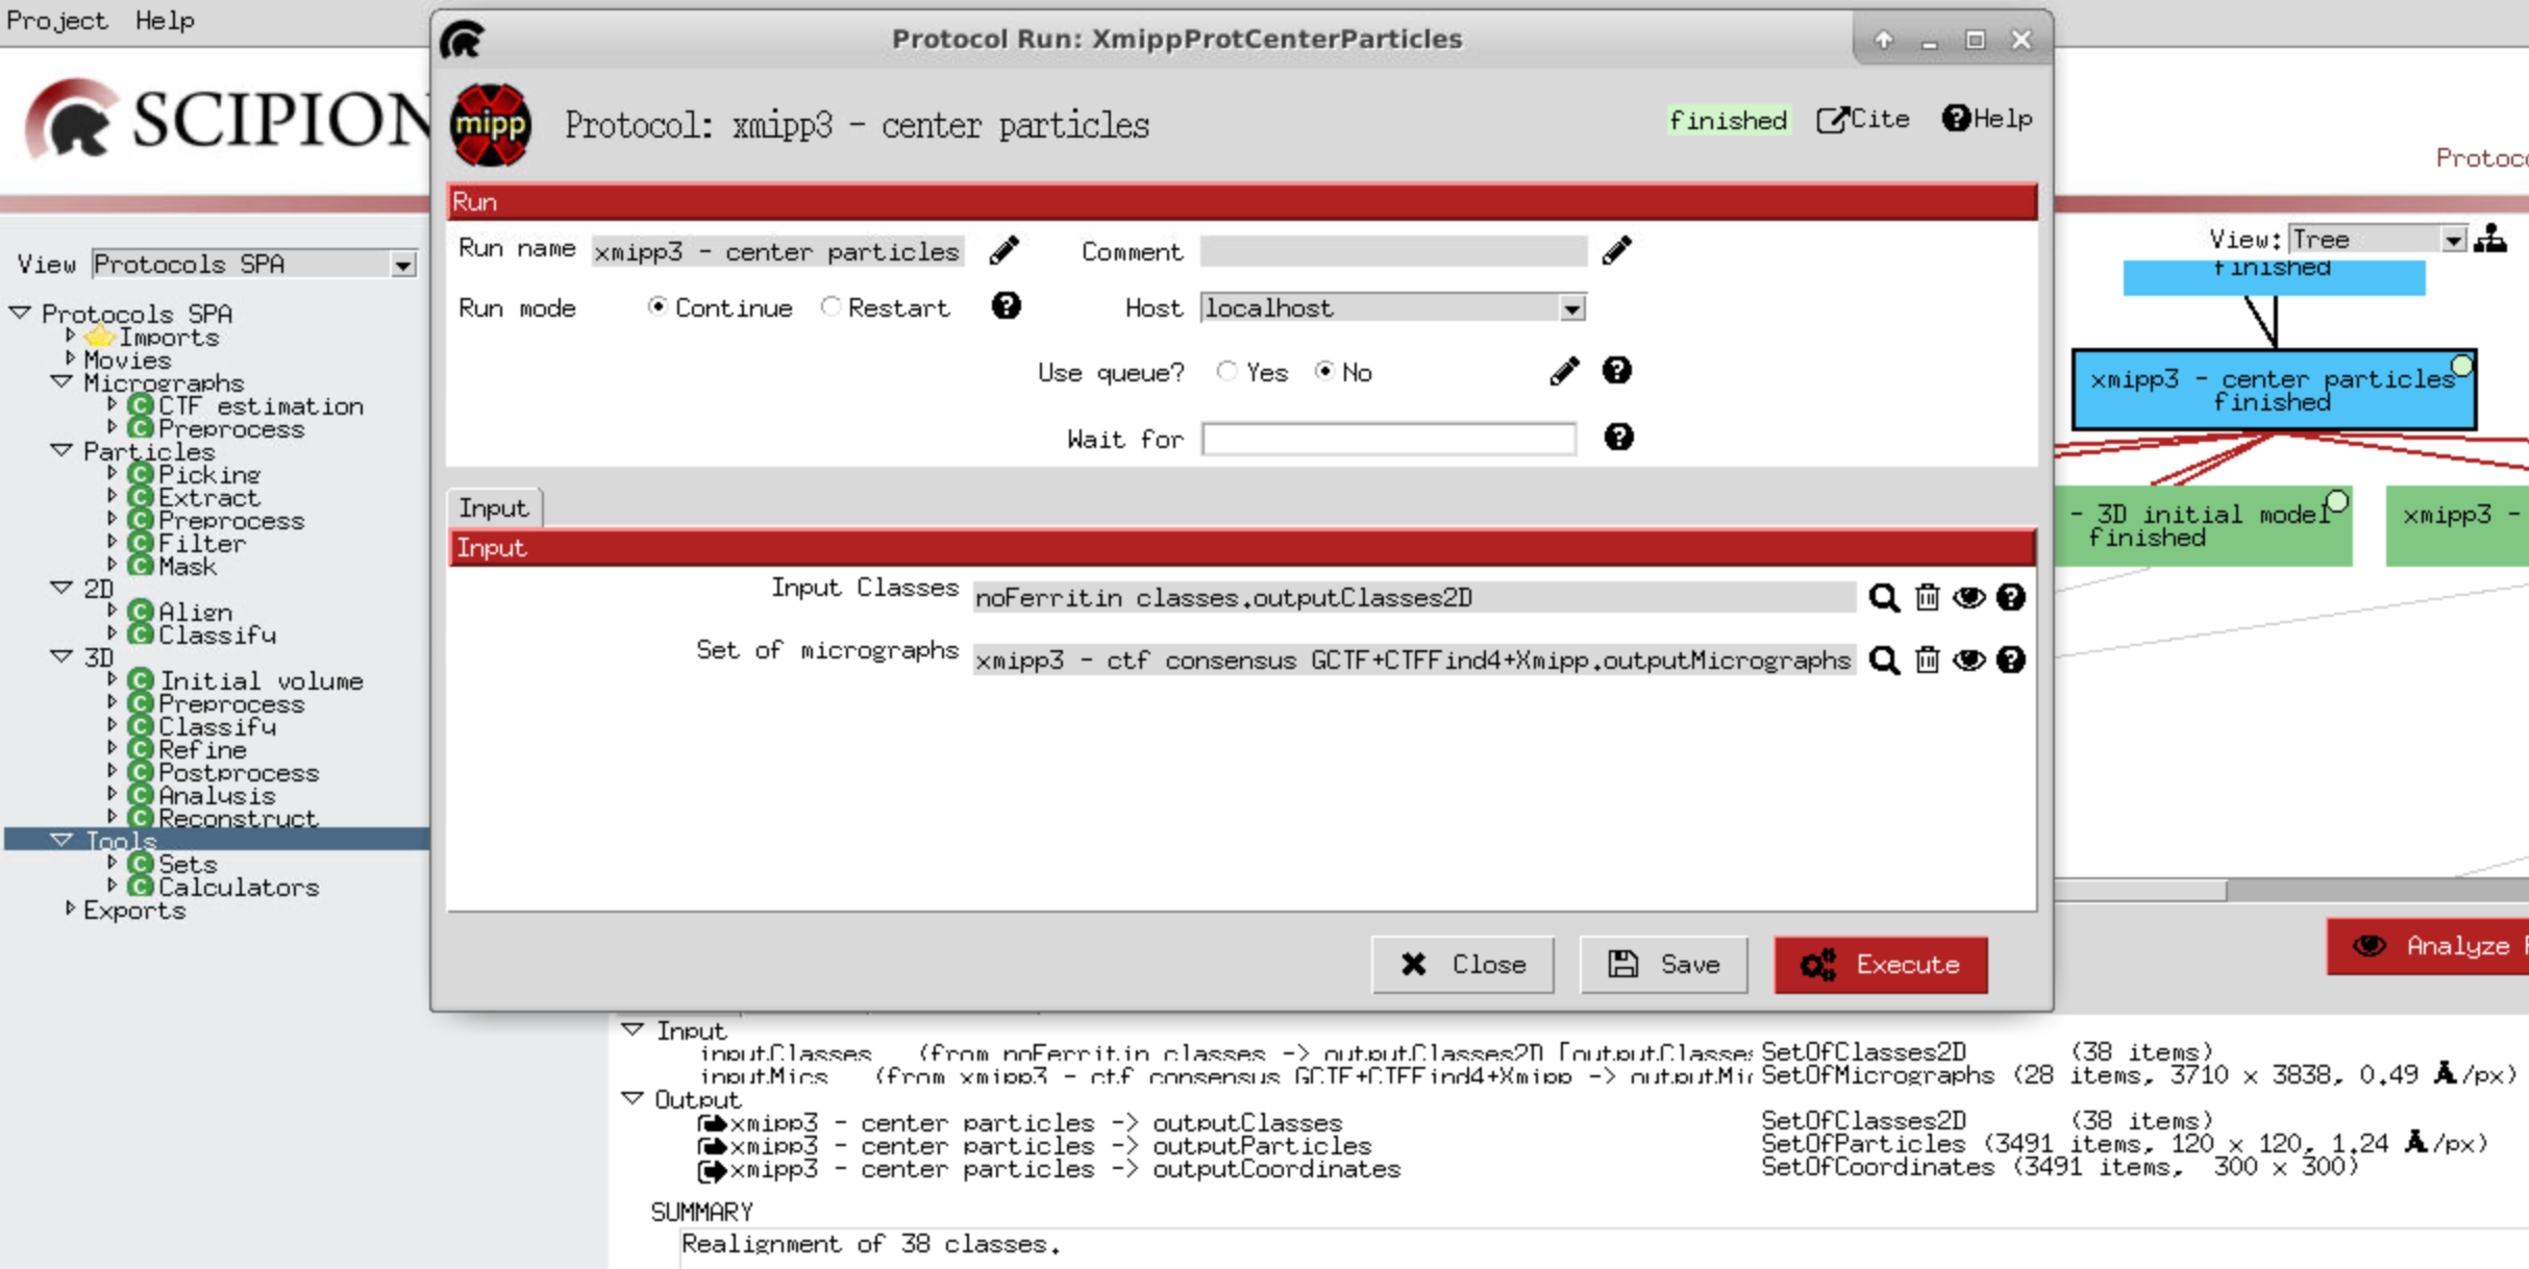
\includegraphics[width=0.95\textwidth]
  {images/7c_xmipp3_centerparticles.pdf}
  \caption{Centering of particles selected in \ttt{noFerritin classes} box.}
  \label{fig:xmipp3_centParticles}
  \end{figure}

This operation will allow us to compute better the initial volumes and also to eliminate duplicates with \scommand{xmipp3-remove duplicates} protocol, as with the recentered particles we can have a better estimate of which are the coordinates that are pointing to the same particle within a radius x (defined to 100).

\begin{figure}[H]
  \centering
  \captionsetup{width=.8\linewidth} 
  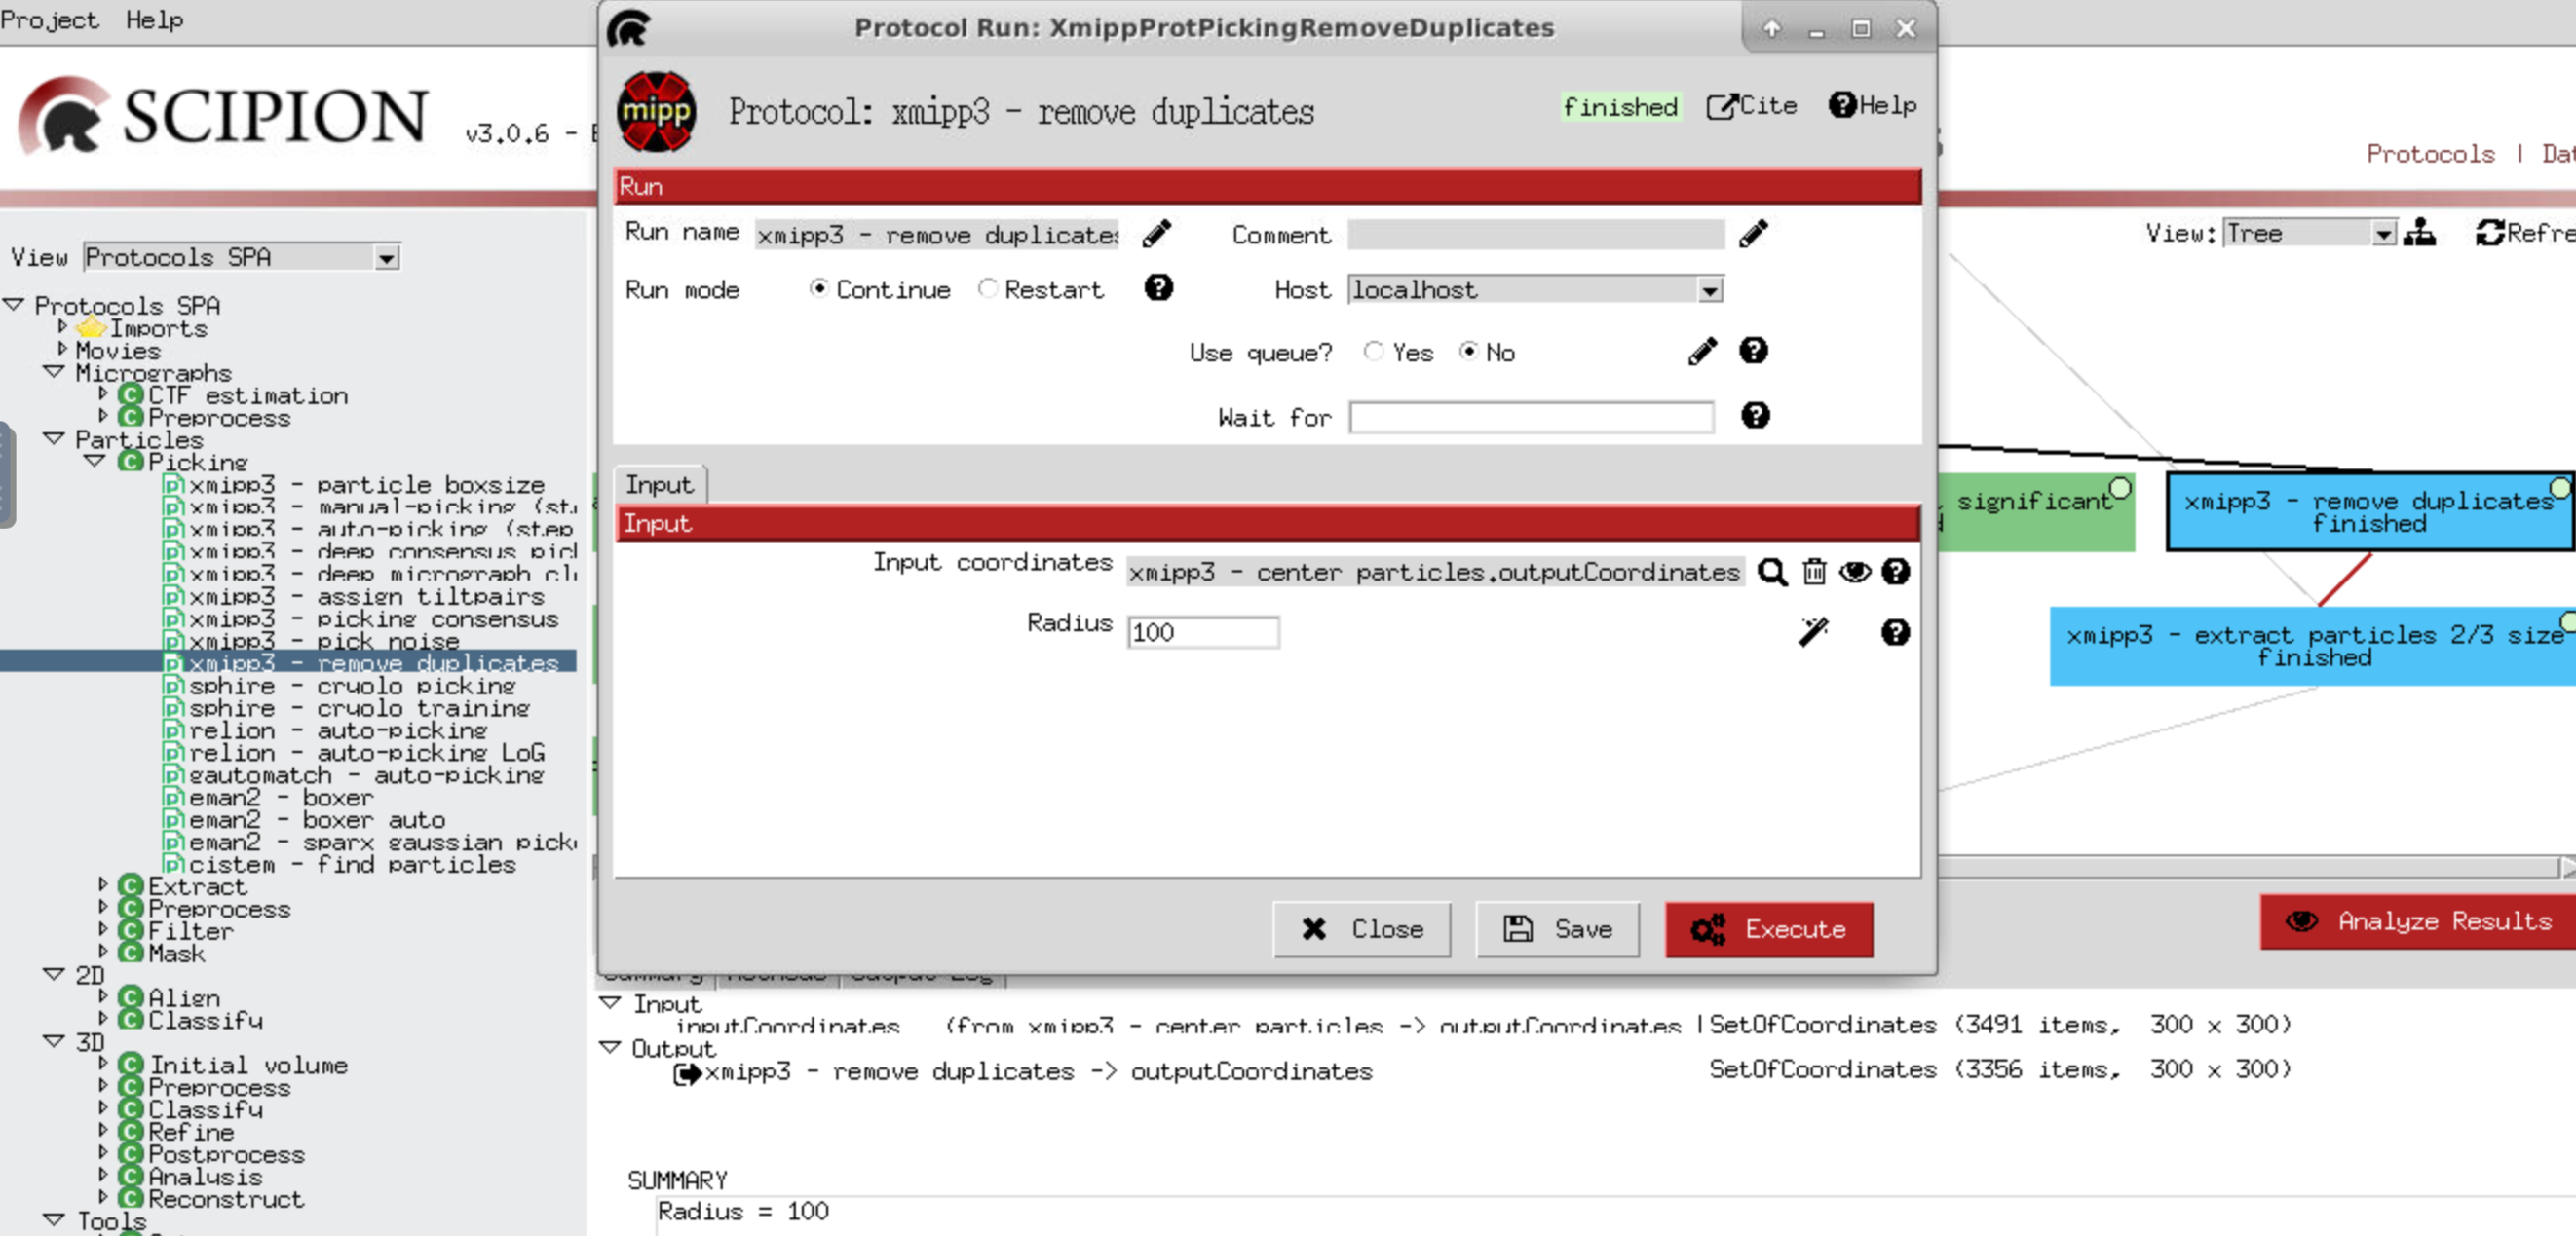
\includegraphics[width=0.95\textwidth]
  {images/7d_xmipp3_removeduplicates.pdf}
  \caption{Remove duplicates from the recentered set of particles.}
  \label{fig:xmipp3_removeDup}
  \end{figure}
  
After running the protocol, particles can be visualized selecting the \scommand{Analyze Results}. In principle, we do not see many overlapping particles in the micrographs. In this case, for 3491 particles 141 were duplicated obtaining a clean set of coordinates of 3,356 particles.\\

Once we have a set of non-duplicated coordinates, we can proceed to extract particles with \ttt{Xmipp} protocol \scommand{xmipp3-extract particles} (\ffigure{fig:xmipp_extract_particles2}). This protocol allows to extract, normalize and correct the CTF phases of the selected particles. As input, this protocol requires the set of coordinates and the consensus CTF values obtained in previous steps, and a downsampling factor 1.5 to obtain more or less 1 A per pixel resolution and 250 box size to correct the CTF effect.

\begin{figure}[H]
  \centering
  \captionsetup{width=.8\linewidth} 
  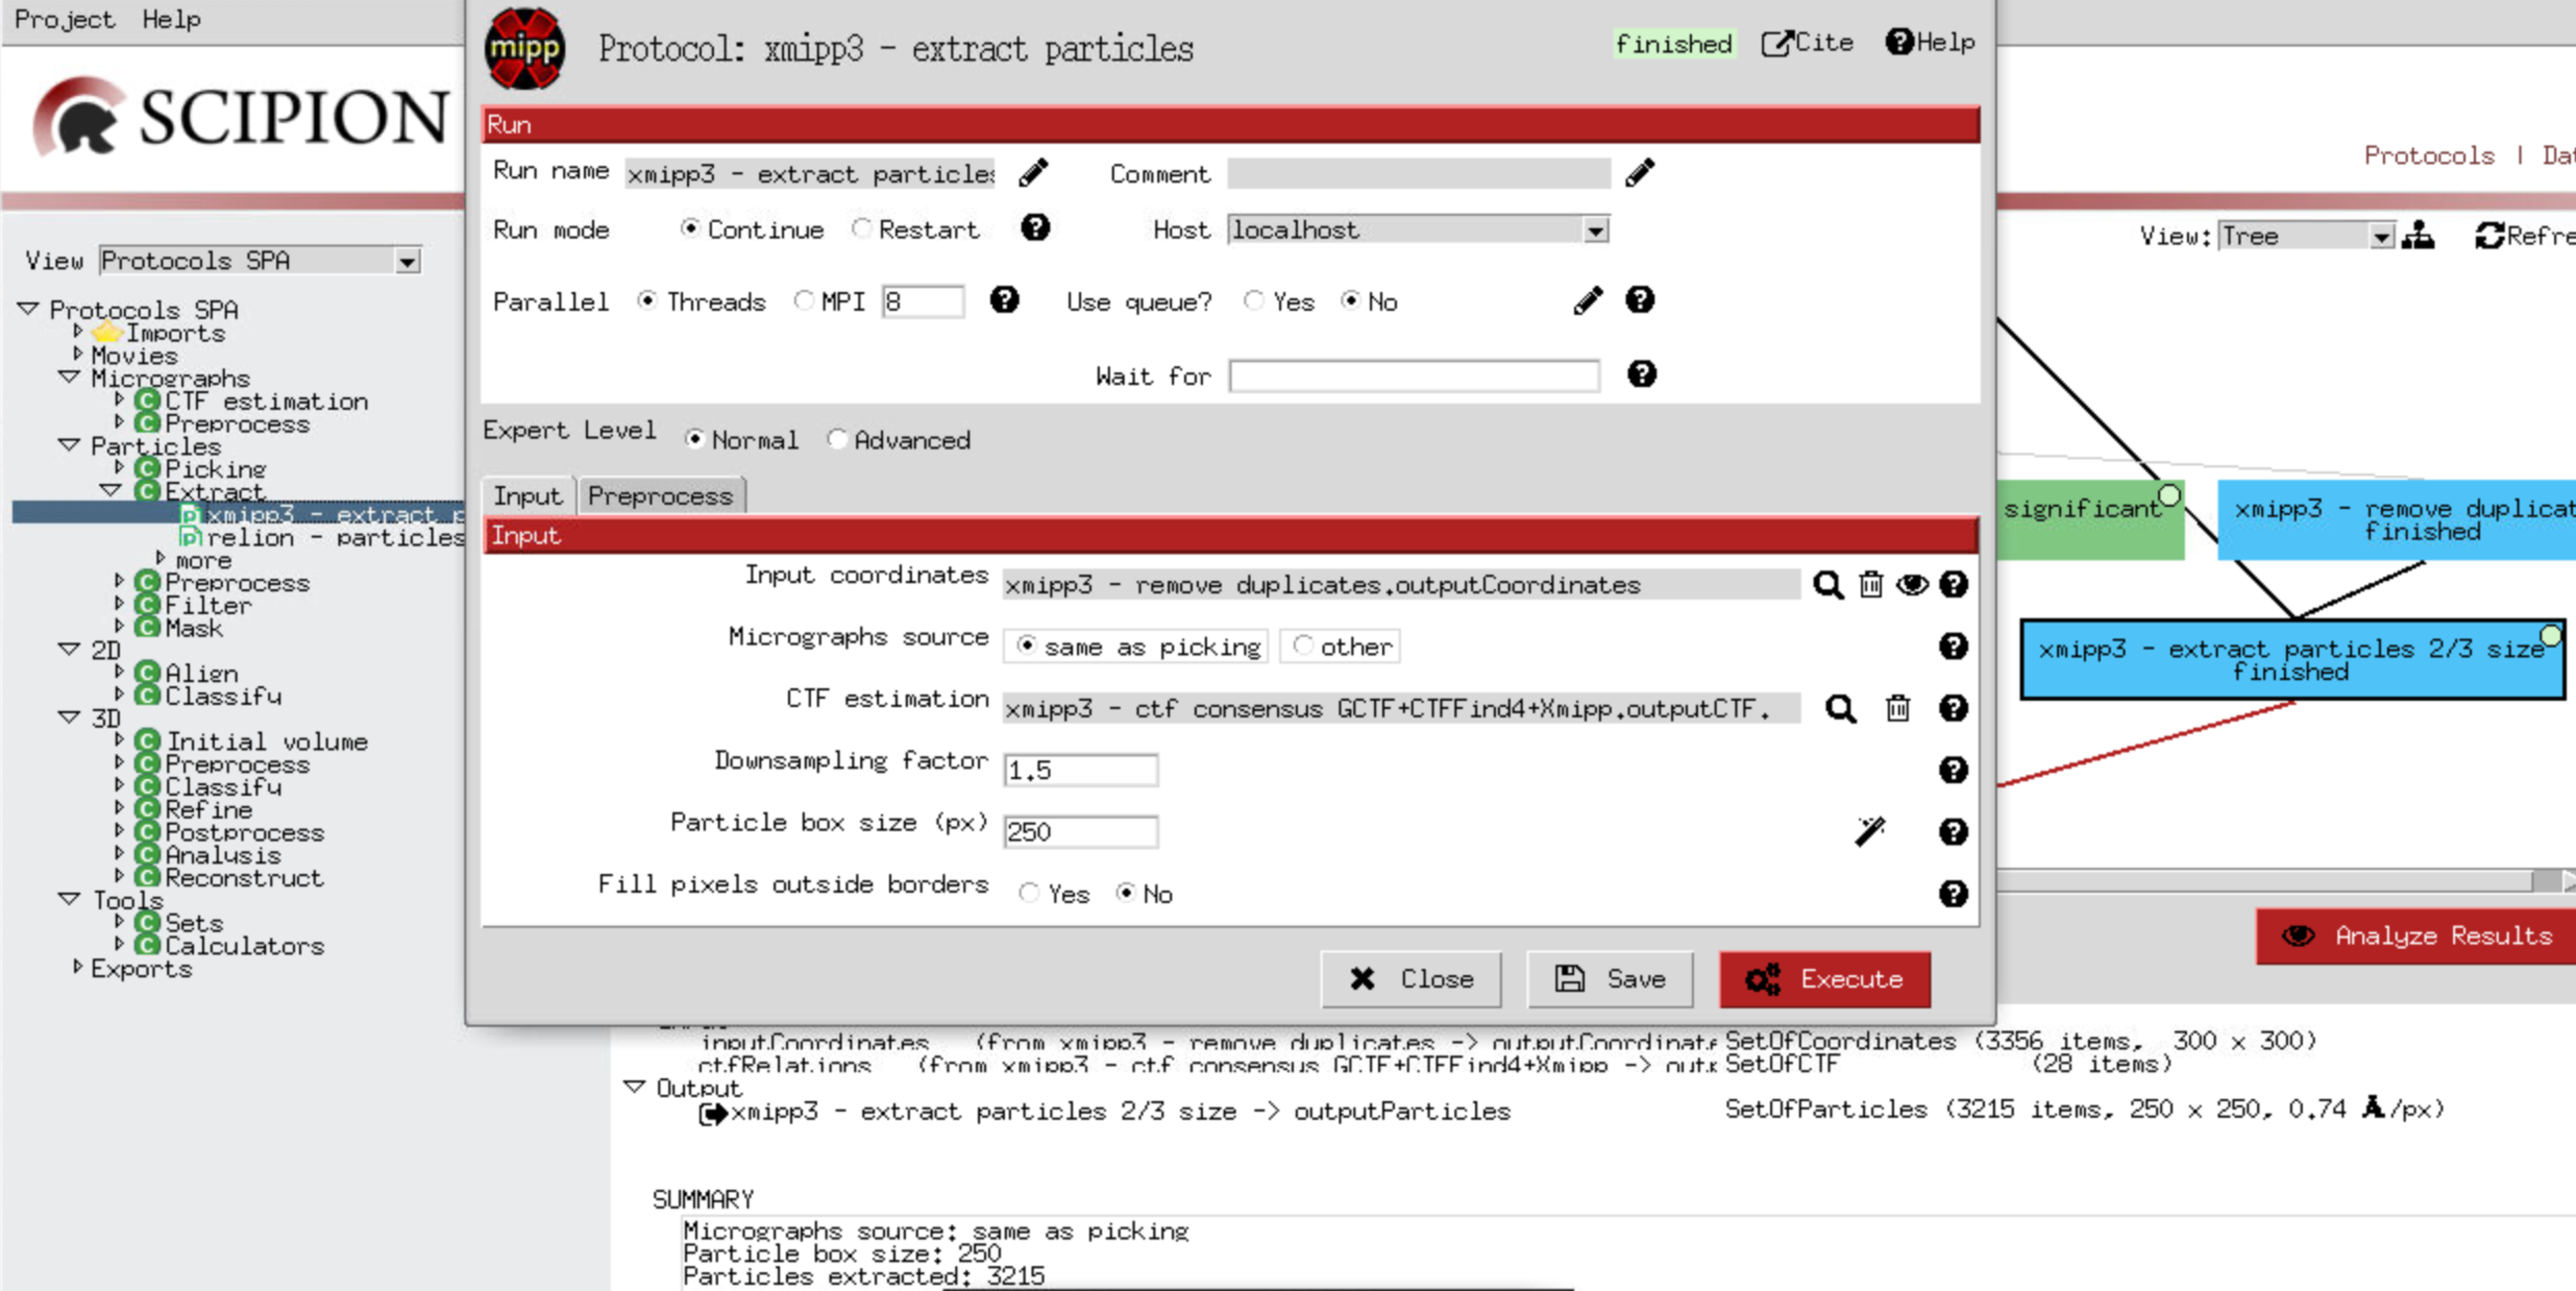
\includegraphics[width=0.95\textwidth]
  {images/7e_xmipp3_extractparticles.pdf}
  \caption{Filling protocol \scommand{xmipp3-extract particles}.}
  \label{fig:xmipp_extract_particles2}
  \end{figure}

The recentered set of particles will be used in the next step in the processing workflow to generate the initial volume and the extracted non-duplicated set of particles will be used in the step in the processing workflow as input of the 3D Refinement and Classification. \\ 

  For more information: 
\begin{itemize}
   \item \textbf{Video tutorial}:  second half of this video \url{https://www.youtube.com/watch?v=eVjQoZ8eohw&list=PLQjWIcrmtc4JjyC-_BM99_XW-VsDa4_i3&index=27}.
   \item \textbf{Theoretical lecture}: second half of this video \url{https://www.youtube.com/watch?v=yVFvN2T_soQ&list=PLQjWIcrmtc4JjyC-_BM99_XW-VsDa4_i3&index=33}.
  \end{itemize}
